%!TEX root = ../Pflichtenheft.tex

\chapter{Zielbestimmung}\label{chap:zielbestimmung}

Die Aufgabe besteht darin, eine plattform\"ubergreifende, interaktive Spielesoftware zu entwickeln, um den
Studenten der Pflichtveranstaltung „Relationale Datenbanksysteme I (RDBI)“ den Umgang mit
der Datenbankanfragesprache SQL vorlesungsbegleitend spielerisch zu vermitteln.

Es soll eine M\"oglichkeit geschaffen werden, praktische Aspekte im Bereich der Datenbankanfragen zu \"uben, da dies im Rahmen 
einer Lehrveranstaltung viele verschiedene Schwierigkeiten mit sich bringt. Zum Einen kann theoretisches Verst\"andnis zwar gut vermittelt werden, 
jedoch ist es nur eingeschr\"ankt m\"oglich, gen\"ugend \"Ubungsmaterial zur Verf\"ugung zu stellen, damit eine komplexe Anfragesprache, wie 
SQL, ge\"ubt und somit auch verstanden werden kann.
Um diese Probleme zu beheben soll die Software mit Fokus auf einen interaktiven SQL-Trainer entwickelt werden. Dieser wird
in zwei verschiedene Spiel-Modi integriert.

Die f\"ur die Applikation gew\"ahlte Sprache ist Englisch. Deshalb werden im folgenden Programmablauf alle spielbezogenen Begriffe 
ebenfalls in englisch benannt. 
 
\section{Registrierung} 
Vor dem ersten Start der Anwendung muss eine Registrierung des Users erfolgen. Daf\"ur steht ein „Sign In“-Fenster
zur Verf\"ugung, das einen Benutzernamen, ein Passwort, sowie eine E-Mail-Adresse oder f\"ur Studenten der TU Braunschweig 
die entsprechende y-Nummer verlangt. Diese Daten werden \"uber eine gesicherte Leitung an das Back-End 
gesendet und dort wird  zwischen y-Nummer und der E-Mail-Adresse unterschieden. Meldet sich der User mit einer E-Mail-Adresse an, so wird 
eine Best\"atigungsanfrage inklusive Aktivierungslink an diese gesendet. Best\"atigt der User die Registrierung, wird ein Userprofile-Object erstellt 
und in der Datenbank gespeichert. Ist der User Student, so wird direkt, ohne Best\"atigung der y-Nummer, das Userprofile-Object gesichert. Eine 
Best\"atigung ist in diesem Fall nicht n\"otig, da der User direkt \"uber das LDAP der Technischen Universit\"at Braunschweig verifiziert wird.

Ist die Registrierung abgeschlossen, wird der Nutzer zum „Login“-Fenster umgeleitet, wo er sich nun mit den vorher registrierten Daten anmelden 
kann. Hierbei reicht die y-Nummer beziehungsweise die E-Mail-Adresse und das Passwort. Die eingegebenen Daten werden mit denen in der 
Datenbank abgeglichen. Ist dies erfolgreich, so gelangt der User in das Hauptmen\"u.

Im Hauptmen\"u besteht die M\"oglichkeit aus folgenden Punkten zu w\"ahlen:

\begin{itemize}
	\item Profile
	\item Story-Mode
	\item Trivia-Mode
	\item Shop
	\item Homework
	\item Leaderboard
	\item Settings 
\end{itemize}

\section{Spielerprofil}
Das Spielerprofil beschreibt alle Nutzereigenschaften und soll dazu dienen eine \"Ubersicht \"uber diese darzustellen. M\"ochte der Spieler diese
eventuell ver\"andern, so muss er in den Reiter Settings wechseln um die Ver\"anderung vorzunehmen.

W\"ahlt der Benutzer nun „Profile“ aus, dann bekommt er einen Einblick \"uber die Benutzerinformationen und die aktuellen pers\"onlichen 
Statistiken. Diese Informationen werden vom Front-End angefragt und vom Back-End zur Verf\"ugung gestellt. \"Ubergeben wird hierbei das bei der 
Registration erstellte Userprofile-Object.
Die pers\"onlichen Statistiken beinhalten:

\begin{itemize}
	\item Den Punktestand im Story- und Trivia-Mode, welcher der akkumulierten Punktezahl aus den gesammelten Lofi-Coins und der Beantwortung eines 
	Statements entspricht. Hierbei bringen schwierigere Statements entsprechend mehr Punkte. Pro Lofi-Coin gibt es generell einen Punkt. Sind die Lofi-Coins in 
	tieferen Stufen des Dungeons gesammelt worden, so wird der Wert des Lofi-Coins mit der erreichten Stufe im Dungeon multipliziert.  		
	\item Den prozentualen Spielerfortschritt im Story-Mode.
	\item F\"ur den Fall, dass der Benutzer den Story-Mode mindestens einmal abgeschlossen hat, wird die geringste Anzahl an Durchg\"angen 
	dargestellt.
	\item Die insgesamt verbrachte Zeit in den jeweiligen Modi. Die Zeit wird ab einer Abwesenheit von 2 Minuten nicht mehr mitberechnet.
	\item Die prozentuale Erfolgsquote des Benutzers beim Beantworten von SQL-Statements.	
	\item Die gesamte Anzahl, sowie der aktuelle Stand an Lofi-Coins im Besitz des Benutzers.
	\item Das f\"ur den Tag festgelegte Limit an Lofi-Coins/Scrolls, die noch vom Benutzer eingesammelt werden k\"onnen.
\end{itemize}
							
\section{Story-Modus}
Der Story-Modus ist der Spielmodus der dem Spieler die M\"oglichkeit bieten soll SQL in einer nicht ganz so trockenen, langweiligen Umgebung zu
\"uben. Der Modus besteht demnach aus einer Mischung aus SQL-Trainer und einem Minispiel. Das Minispiel soll hierbei als 
Motivationsf\"orderung dienen.

Wird nun der „Story-Mode“ gew\"ahlt, wird eine Anfrage an das Back-End gesendet, der Story-Content geladen und der Benutzer gelangt in das 
„Laboratory“. Der Story-Content beinhaltet s\"amtliche Spieldaten. Darunter befinden sich das Inventory, die Playerstatistics, die Scroll-/Lofi-Coin-Limits, 
die Scenetexts und die Scrollcollection (Erkl\"arungen zu diesen Begriffen finden sich im Glossar). Die einzelnen Elemente, die sich im Laboratory 
befinden, sind: Das Character-Sheet, der Belt, die Scrollcollection, der Eingang in das Dungeon und der Ausgang, mit dem der Story-Mode 
verlassen werden kann.

Das Dungeon stellt das Minispielelement der Applikation dar und wird durch einen Endless-Runner repr\"asentiert. Dort werden dem Benutzer die 
verbliebene Anzahl seiner Leben, der Inhalt seines Belts und sein aktueller Punktestand angezeigt. Punkte erh\"alt man durch das Einsammeln von 
M\"unzen und durch das Abschlie{\ss}en von Maps. Diese Maps werden zuf\"allig, aber nach Schwierigkeitsgrad sortiert, von der Spielfigur 
durchlaufen. Nach jeder f\"unften Map gibt es eine Herausforderung, die ohne das Einsetzten von Potions, was wiederum das Bearbeiten von SQL-
Anfragen einschlie{\ss}t, nicht bestanden werden kann. Je tiefer der Spieler in das Dungeon gelangt, desto schwieriger werden die L\"aufe und die 
Anfragen.  

Die Spielfigur besitzt vier Attribute: Jump (Sprungh\"ohe), Speed (Laufgeschwindigkeit), Defense (Verteidigung) und Health (Lebenspunkte). 
Typische Hindernisse, die im Dungeon zu \"uberwinden sind, sind Schluchten, die mit Jump oder Speed \"uberwunden werden k\"onnen und 
kleinere Gegner, die der Spielfigur bei Kollision Health stehlen, wenn nicht genug Defense vorhanden ist. Attribute k\"onnen dauerhaft durch 
„Enchantments“ erh\"oht werden. Daf\"ur m\"ussen vorher entsprechende Scrolls im Dungeon gesammelt werden.
Der Belt repr\"asentiert den G\"urtel der Spielfigur. Dieser hat mehrere Slots, die mit den verschiedenen Potions gef\"ullt werden k\"onnen. Potions 
sind Tr\"anke, die sich der Benutzer brauen kann, wof\"ur er, wie bei den Enchantments zun\"achst eine Scroll im Dungeon finden muss (die 
verschiedenen Scrolls unterscheiden sich hierbei in ihrer Farbgebung, dabei ist die Enchantment-Scroll ist mit einem roten B\"andchen gekennzeichnet). 
F\"ur jede Potion gibt es exakt eine Scroll, die so gesehen ein Rezept darstellt. Die Scrolls werden beim Brauen von Potions nicht verbraucht und 
werden in der Scrollcollection im Laboratory gesammelt. 

Die Scrollcollection ist ein Rezeptbuch, in dem sich alle zur Verf\"ugung stehenden Scrolls, Enchantments und Potions sammeln. W\"ahlt man eine 
Scroll aus, fordert das Front-End eine SQL-Anfrage von dem Back-End. Daraufhin liefert das Back-End einen Task, der aus einer Fragestellung und 
einem Datenbankschema besteht, aus. %wie wird es dargestellt?
Der Spieler beantwortet die Anfrage, sie wird zur\"uck an das Back-End gesendet, wird auf Korrektheit 
\"uberpr\"uft  und inklusive eines Fehlerhinweises zur\"uckgeschickt. Der Fehlerhinweis wird so umschrieben, dass die M\"oglichkeit f\"ur 
den Spieler besteht seine Anfrage zu korrigieren. Beantwortet der Spieler sie korrekt, erh\"alt er die entsprechende Potion, beziehungsweise das 
Enchantment. Die Schwierigkeit des Tasks ist abh\"angig von der Scroll. Je tiefer die Scroll im Dungeon gefunden worden ist, sprich wie weit der 
Spieler in der Story fortgeschritten ist, desto schwieriger ist der Task. 
Au{\ss}erdem erh\"alt der Benutzer Lofi-Coins f\"ur das richtige Bearbeiten der Anfrage. Hierbei ist die Anzahl der erhaltenen Lofi-Coins abh\"angig vom 
Schwierigkeitsgrad und der Bearbeitungszeit. Die Ver\"anderungen von Inventory und Lofi-Coin-Guthaben wird im Back-End gesichert.
Das Character-Sheet zeigt den zurzeit ausgew\"ahlten Avatar und die Werte der oben beschriebenen Attribute des Spielers.

\section{Tutorial}
Beim ersten Aufruf des Story-Modes wird ein „Tutorial“ gestartet, welches verlustfrei \"ubersprungen werden kann. Das gesamte Tutorial wird durch 
den narrativen Charakter des Spiels, einem raubeinigen Zauberschrank namens „Secreterry“, gehalten. Dieses Tutorial besteht aus einer Einf\"uhrung 
der einzelnen oben genannten Elemente des Laboratory und der Erkl\"arung eines Spielablaufes. Hierbei werden die einzelnen Elemente 
visuell hervorgehoben und sowohl auditiv, als auch textuell beschrieben. Diese Informationen werden nach Anfrage direkt zu Anfang mit dem Story-
Content \"uber das Back-End geladen. Nachdem alle Elemente erkl\"art worden sind, wird dem Benutzer ein festgelegter Teil des Minispiels erkl\"art. 
Dieses beginnt mit einem ersten Lauf durch das Dungeon. In einer vorgefertigten Tutorial-Map erh\"alt der Benutzer eine erste Scroll und st\"o{\ss}t auf ein, zu diesem Zeitpunkt, un\"uberwindbares Hindernis und stirbt. Daraufhin erscheint ein „Game-Over“-Screen, in dem die 
eingesammelten Items aufgelistet werden, in diesem Fall eine Scroll, mit der der Spieler in der Lage ist eine Jump-Potion zu brauen. Nun f\"uhrt 
das Tutorial zur\"uck in das Laboratory und zeigt dem Benutzer wie die gesammelte Scroll in der Scrollcollection benutzt werden kann um die 
Potion zu brauen, sprich der Spieler beantwortet eine einfache SQL-Anfrage und bekommt seine Potion. Im n\"achsten Schritt des Tutorials wird 
dem Spieler durch Secreterry erkl\"art, wie die Potion in den Belt eingef\"ugt wird. Dazu wechselt der Benutzer in das Untermen\"u Belt, wo er die 
Potion ausw\"ahlt und in einen der daf\"ur vorgesehenen Slots einf\"ugt. Nun ist der User in der Lage das vorher genannte un\"uberwindbare 
Hindernis zu bew\"altigen. Am Ende dieses Levels erh\"alt er eine weitere Scroll, welche diesmal das Rezept f\"ur ein Enchantment enth\"alt. 

Wenn das Tutorial erfolgreich beendet, beziehungsweise \"ubersprungen, wurde stellt das Front-End die Anfrage an das Back-End den n\"achsten 
Part der Story inklusive Spieldaten zu laden. Dieser, wie auch alle folgenden, besteht wieder aus dem aktuellen Inventory, den Playerstatistics, den 
(nun aktualisierten) Scroll-/Lofi-Coin-Limits, den jeweiligen Scenetexts und der Scrollcollection. Jeder Teil der Story besteht aus einer Einf\"uhrung durch 
den narrativen Charakter, die dem Benutzer den aktuellen Stand des Spieles erl\"autert, mit Bezug auf den vorherigen Teil des Spieles. Durch 
weitere Durchl\"aufe im Dungeon, das Einsammeln der Scrolls und das Benutzen dieser, ist der Benutzer in der Lage weitere Parts zu laden und 
immer weiter im Dungeon vorzudringen, bis man schlie{\ss}lich nach acht Parts zum Endgegner gelangt.
Zuletzt sei zu erw\"ahnen, dass der Benutzer zu jeder Zeit den Story-Mode verlassen kann, wobei sein Fortschritt und sein Inventory im Back-End 
gespeichert werden.

Zur Veranschaulichung des gesamten Spielablaufes inklusive Tutorial dient eine tabellarische Darstellung, die am Ende von Kapitel 1 zu finden ist. 
Diese Darstellung ist ebenfalls in ein Aktivit\"atsdiagramm \"uberf\"uhrt worden. Dieses ist wiederum in Kapitel 3 zu finden.

\begin{figure}[ht]
\centering
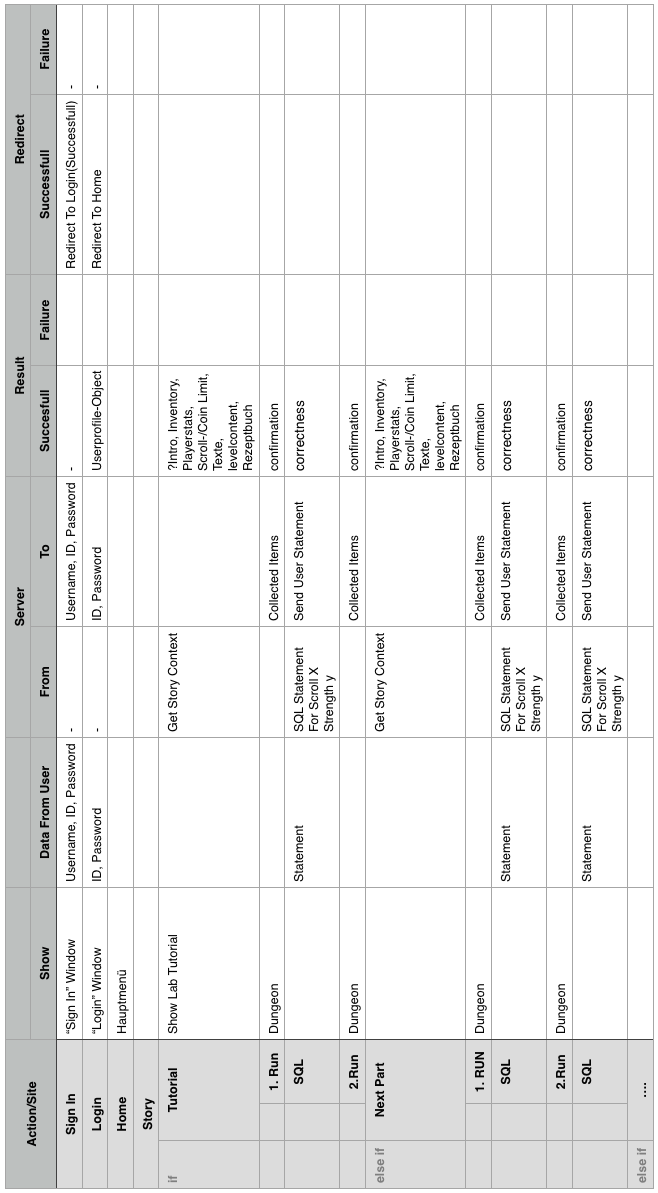
\includegraphics[width=0.75\textwidth]{figures/Spielablauf.PNG}
\caption{Veranschaulichung des Spielablaufes}
\end{figure}

\section{Trivia-Modus}
Der Trivia-Modus ist f\"ur die Spieler, die reines SQL lernen m\"ochten. Dazu kommt der SQL-Trainer zum Vorschein.   

W\"ahlt der Benutzer nun den „Trivia-Mode“ aus, so kann er SQL-Anfragen \"uben, ohne das Minispiel zu spielen. Geladen werden auch hier wieder, 
nach Anfrage durch das Front-End an das Back-End, s\"amtliche daf\"ur ben\"otigten Information. Diese bestehen demnach aus einem gesamten 
Task inklusive Datenbankschema und dem Anfragetext, zu welchem das SQL-Statement erstellt werden muss. Hierbei hat der Spieler von 
vornherein die M\"oglichkeit  einen aus f\"unf Schwierigkeitsgraden auszuw\"ahlen. Hat er sich f\"ur einen Schwierigkeitsgrad entschieden, beginnt 
der gleiche Ablauf, wie bei den Tasks im Story-Mode. Das Front-End schickt eine Anfrage an das Back-End und ein kompletter Task wird 
\"ubergeben. Aber auch in diesem Mode hat der Spieler die M\"oglichkeit, ohne Story-Content in das Dungeon zu gehen und nach Belieben mehr 
oder weniger viele, zuf\"allig ausgew\"ahlte, Maps zu spielen. Daf\"ur wird es einen eigens daf\"ur vorgesehenen Men\"upunkt  geben, mit dem der 
Spieler zu jeder Zeit hin, aber auch wieder zur\"uck wechseln kann.

\section{Shop}
Der Shop dient dazu, den Spielern ein wenig Raum f\"ur Personalisierung zu bieten. 
W\"ahlt der Benutzer „Shop“, wird ihm die M\"oglichkeit gegeben, gesammelte Lofi-Coins gegen Spieler-Avatare einzutauschen, die gleichzeitig die 
Spielfigur im Dungeon repr\"asentieren. Au{\ss}erdem soll es die M\"oglichkeit geben weitere Slots zum Belt der Spielfigur dazu zu kaufen. Auch
weitere Leben k\"onnen hier gegen Lofi-Coins erworben werden. 

\section{Hausaufgaben-Modus} 
W\"ahlt der Spieler „Homework“, so kann er die in der Applikation verkn\"upften Hausaufgaben bearbeiten. Hierbei stellt wieder das Front-End die 
Anfrage an das Back-End. Daf\"ur ist ein komplettes Aufgabenpaket mit unterschiedlich schwierigen SQL-Aufgaben vorgesehen. Die Hausaufgabe 
ist erst dann abgeschlossen, wenn das Aufgabenpaket unter einer bestimmten Abschlussbedingung erf\"ullt worden ist. Die Bedingung kann 
entweder ein Punkte-Limit oder ein Zeit-Limit sein. Ein Aufgabenpaket kann auch aus einer gewissen Anzahl an SQL-Statements bestehen.
Diese Bedingung kann von einem Wissenschaftlichen Mitarbeiter des Dozenten von RDBI f\"ur die w\"ochentlichen Challenges ausgew\"ahlt 
werden und in der Datenbank hinterlegt werden. Der Benutzer hat also nur innerhalb einer Woche Zeit das gesamte Aufgabenpaket zu l\"osen, 
erst dann wird die Hausaufgabe als abgeschlossen markiert.  Auch die Aufgabenstellung und die Statements der zu l\"osenden Aufgaben m\"ussen von dem 
Mitarbeiter in die Datenbank eingef\"ugt werden. Daf\"ur steht das Admin-Tool des Back-Ends zur Verf\"ugung. Ist ein Aufgabenpaket f\"ur eine 
bestimmte Woche erstellt worden, so kann sie von einem Studenten bearbeitet werden. W\"ahlt der Student die aktuelle Hausaufgabe aus, 
geht die Anfrage f\"ur eine erste Aufgabenstellung raus und das Back-End sendet die Aufgabe zur\"uck.

Schickt der Benutzer einmal ein Statement ab, so wird auch hier wieder eine Kontrolle durchgef\"uhrt und mit eventuellem Fehlerhinweis zur\"uckgeschickt. 
Der User korrigiert sein Statement und sendet es erneut an das Back-End. Bei richtiger Beantwortung wird dieses Statement als 
abgeschlossen markiert und auf dem Server gesichert. Bevor die Aufgaben jedoch gel\"ost werden k\"onnen, m\"ussen sie in das Back-End eingepflegt 
werden. Daf\"ur steht das Admin-Tool zur Verf\"ugung. Dort kann auch jeder Student nachschauen ob er die Hausaufgaben, beziehungsweise die 
Challenges, bestanden hat oder nicht.


\section{Admin-Tool}
Das Admin-Tool stellt f\"ur verschiedene Benutzergruppen unterschiedliche Funktionen zur Verf\"ugung. Studenten, die sich mit ihrer y-Nummer registriert haben,
k\"onnen hier die Ergebnisse aller von ihnen bearbeiteten Hausaufgaben einsehen. Wenn ein Spieler die vom Kunden gew\"unschten Kriterien erf\"ullt hat, k\"onnen 
diese „bef\"ordert“ werden. Einem bef\"orderten Benutzer ist es m\"oglich selbst Aufgaben zu erstellen, die von anderen Spielern im Trivia-Mode bearbeitet werden k\"onnen, 
wenn sie diese Funktion wahrnehmen m\"ochten. Dieses kann jeder Spieler f\"ur sich entscheiden und im Men\"u im Trivia-Mode die daf\"ur vorgesehene Checkbox aktivieren.
Des Weiteren gibt es die Gruppe der Administratoren. Diese sind vor allem f\"ur die Benutzerverwaltung verantwortlich. Sie k\"onnen Benutzer l\"oschen, Challenge-Pakete 
und Hausaufgaben erstellen, sowie die L\"osungen der Studenten einsehen.

\section{Einstellungen}
Wählt der Benutzer „Settings“ hat er Zugriff auf allgemeine Einstellungen. Diese werden Spieler-spezifisch im Back-End gespeichert und beim Aufruf 
von diesem erfragt. Der User hat nun die folgenden Einstellungsmöglichkeiten:
\begin{itemize}	
	\item Sound on/off: Aktiviert oder deaktiviert die Soundeffekte die beim Springen der Spielfigur oder beim Bet\"atigen eines Buttons abgespielt werden.
	\item Music on/off: Aktiviert oder deaktiviert die Hintergrundmusik des Minispiels.
	\item Tutorial: Das Tutorial kann reaktiviert werden, damit die Spieler, die es vermeidlich \"ubersprungen haben, dieses trotzdem nochmal ansehen k\"onnen. 
	\item Story-Reset: Setzt den Fortschritt des Story-Modes nach zurück. Dieses muss best\"atigt werden.
	\item Change Username: Gibt dem User die Möglichkeit, seinen Benutzernamen zu ändern.
	\item Change Password: Gibt dem User die Möglichkeit, sein Passwort zu ändern.
	\item Delete Profile: Hiermit kann der User sein komplettes Profil l\"oschen.
\end{itemize}	
Erfolgt eine Änderung der Einstellungen, wird diese sofort ans Back-End geschickt, dort gespeichert und kurz darauf im Front-End aktualisiert.
	
	
\section{Ranglisten}
Die Leaderboards dienen zus\"atzlich zu dem Minispiel als Motivationsf\"orderung.
Wählt der Benutzer „Leaderboards“ bekommt er eine Einsicht in Ranglisten, in denen die Statistiken aller Benutzer in den verschiedenen Modi dargestellt werden.
Folgende Ranglisten gibt es sowohl für den „Story-Mode“ als auch für den „Trivia-Mode“:
\begin{itemize}	
	\item Gesamtanzahl Lofi-Coins (total lofi-coins)
	\item Gesamtanzahl Läufe (total runs)
	\item geringsten Anzahl an benötigten Durchgängen für die Story (min. runs per story)
	\item insgesamt im Spiel verbrachten Zeit (time spent)
	\item Anzahl an abgeschlossenen Stories (story count)
	\item prozentuale Erfolgsquote beim Beantworten von Anfragen
	\item prozentuale Erfolgsquote der beim ersten Versuch korrekt beantworteten Anfragen
\end{itemize}
	
Die „Top Ten“ jeder dieser Ranglisten werden direkt als Liste dargestellt. Ist der Benutzer unter diesen, wird er markiert, falls nicht, wird sein Rang unter dieser 
Liste angezeigt. Der Benutzer hat die Möglichkeit sowohl seinen eigenen Rang, als auch den anderer Benutzer zu sehen, sofern er deren Benutzernamen kennt. 
Die Daten für die Ranglisten werden vom Back-End zusammengestellt und auf Anfrage ans Front-End gesendet.


\section{Musskriterien}\label{sec:musskriterien}
\must{1}{Es wird ein „Jump\&Run“-Minispiel f\"ur die Motivationsf\"orderung der User geben.}
\must{2}{Ein grafisch aufbereitetes Webinterface, in dem die Men\"uf\"uhrung eingebettet ist.}
\must{3}{Ein SQL-Trainer, das aus einem Aufgabenstellungsfenster und einem Eingabefenster besteht.}
\must{4}{Das Back-End wird entsprechende Nutzerdaten der Spieler speichern, sichern.}
\must{5}{Das Back-End wird ein Admin-Tool zur Userverwaltung zur Verf\"ugung stellen.}
\must{6}{Das Back-End wird ein Admin-Tool zur Aufgabenverwaltung zur Verf\"ugung stellen.}
\must{7}{Es wird die drei verschiedenen Spielmodi geben (Trivia-, Story und Homework-Mode).}
\must{8}{Die Software wird an das LDAP der Technischen Universit\"at Braunschweig angebunden.}
\must{9}{Die Game-Engine ist in das Back-End integriert.}


\section{Sollkriterien}\label{sec:sollkriterien}
\should{1}{Das Minispiel kann in verschiedenen Schwierigkeitsgraden gespielt werden.}
\should{2}{Die Applikation soll auf mobilen Endger\"aten ausf\"uhrbar sein.}
\should{3}{Der Avatar, beziehungsweise die Spielfigur sollen ersetzt oder personalisiert werden k\"onnen.}
\should{4}{Es k\"onnen Highscores generiert und im Profil visualisiert werden.}
\should{5}{Auch Leaderboards sollen generiert und in einem eigenen Men\"upunkt visualisiert werden k\"onnen.}


\section{Kannkriterien}\label{sec:kannkriterien}
\could{1}{Es k\"onnten neben den Hausaufgaben-Paketen auch \"Ubungspakete erstellt werden k\"onnen.}
\could{2}{Auch andere Universit\"aten k\"onnten \"uber ein entspechendes LDAP angebunden werden.}
\could{3}{Es k\"onnte ein abgespecktes Tutorial f\"ur den Trivia-Mode geben.}
\could{4}{In den Shop k\"onnten weitere Features integriert werden.} 
\could{5}{Die Steuerung des Minispiel kann auf Tasten, statt Mausklicks gelegt werden.}
\could{6}{Es soll Freundeslisten geben k\"onnen.}


\section{Abgrenzungskriterien}\label{sec:abgrenzungskriterien}
\wont{1}{Die Verkn\"upfung zu Social-Networks soll nicht realisiert werden.}
\wont{2}{Es wird keinen Mode geben, in dem der Fokus nur auf dem Minispiel liegt.}
\wont{3}{Innerhalb der Applikation wird es keine M\"oglichkeit f\"ur In-Game-K\"aufe geben.}
\wont{4}{Es wird keine kostenpflichtigen Zugriffsm\"oglichkeiten f\"ur die Software geben.}
\wont{5}{Es werden keine Hausaufgabenergebnisse in das HMS des Instituts f\"ur Informationssysteme \"ubertragen.}